\documentclass[12pt,letterpaper]{article}
\usepackage{graphicx,textcomp}
\usepackage{natbib}
\usepackage{setspace}
\usepackage{fullpage}
\usepackage{color}
\usepackage[reqno]{amsmath}
\usepackage{amsthm}
\usepackage{fancyvrb}
\usepackage{amssymb,enumerate}
\usepackage[all]{xy}
\usepackage{endnotes}
\usepackage{lscape}
\newtheorem{com}{Comment}
\usepackage{float}
\usepackage{hyperref}
\newtheorem{lem} {Lemma}
\newtheorem{prop}{Proposition}
\newtheorem{thm}{Theorem}
\newtheorem{defn}{Definition}
\newtheorem{cor}{Corollary}
\newtheorem{obs}{Observation}
\usepackage[compact]{titlesec}
\usepackage{dcolumn}
\usepackage{tikz}
\usetikzlibrary{arrows}
\usepackage{multirow}
\usepackage{xcolor}
\newcolumntype{.}{D{.}{.}{-1}}
\newcolumntype{d}[1]{D{.}{.}{#1}}
\definecolor{light-gray}{gray}{0.65}
\usepackage{url}
\usepackage{listings}
\usepackage{color}


\definecolor{codegreen}{rgb}{0,0.6,0}
\definecolor{codegray}{rgb}{0.5,0.5,0.5}
\definecolor{codepurple}{rgb}{0.58,0,0.82}
\definecolor{backcolour}{rgb}{0.95,0.95,0.92}

\lstdefinestyle{mystyle}{
	backgroundcolor=\color{backcolour},   
	commentstyle=\color{codegreen},
	keywordstyle=\color{magenta},
	numberstyle=\tiny\color{codegray},
	stringstyle=\color{codepurple},
	basicstyle=\footnotesize,
	breakatwhitespace=false,         
	breaklines=true,                 
	captionpos=b,                    
	keepspaces=true,                 
	numbers=left,                    
	numbersep=5pt,                  
	showspaces=false,                
	showstringspaces=false,
	showtabs=false,                  
	tabsize=2
}
\lstset{style=mystyle}
\newcommand{\Sref}[1]{Section~\ref{#1}}
\newtheorem{hyp}{Hypothesis}

\title{Applied Stats - Problem Set 3}
\author{Yana Konshyna}


\begin{document}
	\maketitle
	\section*{Instructions}
	\begin{itemize}
		\item Please show your work! You may lose points by simply writing in the answer. If the problem requires you to execute commands in \texttt{R}, please include the code you used to get your answers. Please also include the \texttt{.R} file that contains your code. If you are not sure if work needs to be shown for a particular problem, please ask.
	\item Your homework should be submitted electronically on GitHub.
	\item This problem set is due before 23:59 on Sunday November 19, 2023. No late assignments will be accepted.

	\end{itemize}

		\vspace{.25cm}
	
\noindent In this problem set, you will run several regressions and create an add variable plot (see the lecture slides) in \texttt{R} using the \texttt{incumbents\_subset.csv} dataset. Include all of your code.

\vspace{.5cm}
\section*{Question 1}
\vspace{.25cm}
\noindent We are interested in knowing how the difference in campaign spending between incumbent and challenger affects the incumbent's vote share. 
	\begin{enumerate}
		\item Run a regression where the outcome variable is \texttt{voteshare} and the explanatory variable is \texttt{difflog}.	\vspace{0.5cm}
		
		\lstinputlisting[language=R, firstline=34, lastline=36]{PS3_my answers_YK_23359606.R}  
		\vspace{.25cm}
		
		\noindent \textbf After loading \texttt{incumbents\_subset.csv} dataset into the working environment, I execute the regression model in which the vote share of the presidential candidate of the incumbent's party (\texttt{voteshare}) is explained by the difference in campaing spending between incumbent and challenger (\texttt{difflog}). Then I investigate the estimated coefficients of the model using summary(). \vspace{0.5cm}
	
	\noindent \textbf{Code in R:}
	\lstinputlisting[language=R, firstline=40, lastline=43]{PS3_my answers_YK_23359606.R}  
	\vspace{.25cm}
	
	\noindent \textbf{Output: }
		\begin{footnotesize}
			\begin{verbatim}
	Residuals:     Min       1Q   Median       3Q      Max
            -0.26832 -0.05345 -0.00377  0.04780  0.32749 
Coefficients:            
            Estimate Std. Error t value Pr(>|t|)    
(Intercept) 0.579031   0.002251  257.19   <2e-16 ***
difflog     0.041666   0.000968   43.04   <2e-16 ***
---
Signif. codes:  0 ‘***’ 0.001 ‘**’ 0.01 ‘*’ 0.05 ‘.’ 0.1 ‘ ’ 1
Residual standard error: 0.07867 on 3191 degrees of freedom
Multiple R-squared:  0.3673,	Adjusted R-squared:  0.3671 
F-statistic:  1853 on 1 and 3191 DF,  p-value: < 2.2e-16				
		
	\end{verbatim}  
		\end{footnotesize}


	
	\noindent \textbf{Conclusion:} Increasing the difference in campaing spending between incumbent and challenger by 1 unit, on average, will increase the incumbent's vote share by 0.041 units. The estimated coefficient is statistically differentiable from zero at the  $\alpha=0.05$ level because the p-value $<$ 0.05 ($\approx $2e-16).
	 \vspace{1 cm}
	
				\item Make a scatterplot of the two variables and add the regression line. 	\vspace{0.5cm}
		
		\noindent \textbf Making a scatterplot of the two variables and adding the regression line by using plot() and abline(). \vspace{0.5cm}
		
		\noindent \textbf{Code in R:}
		\lstinputlisting[language=R, firstline=46, lastline=55]{PS3_my answers_YK_23359606.R}  
		\vspace{.25cm}
		
\begin{center}
			\noindent Scatterplot 1 with the regression line.
\end{center}
		
		\begin{figure}[h!]\centering

			\label{fig:plot_1}
			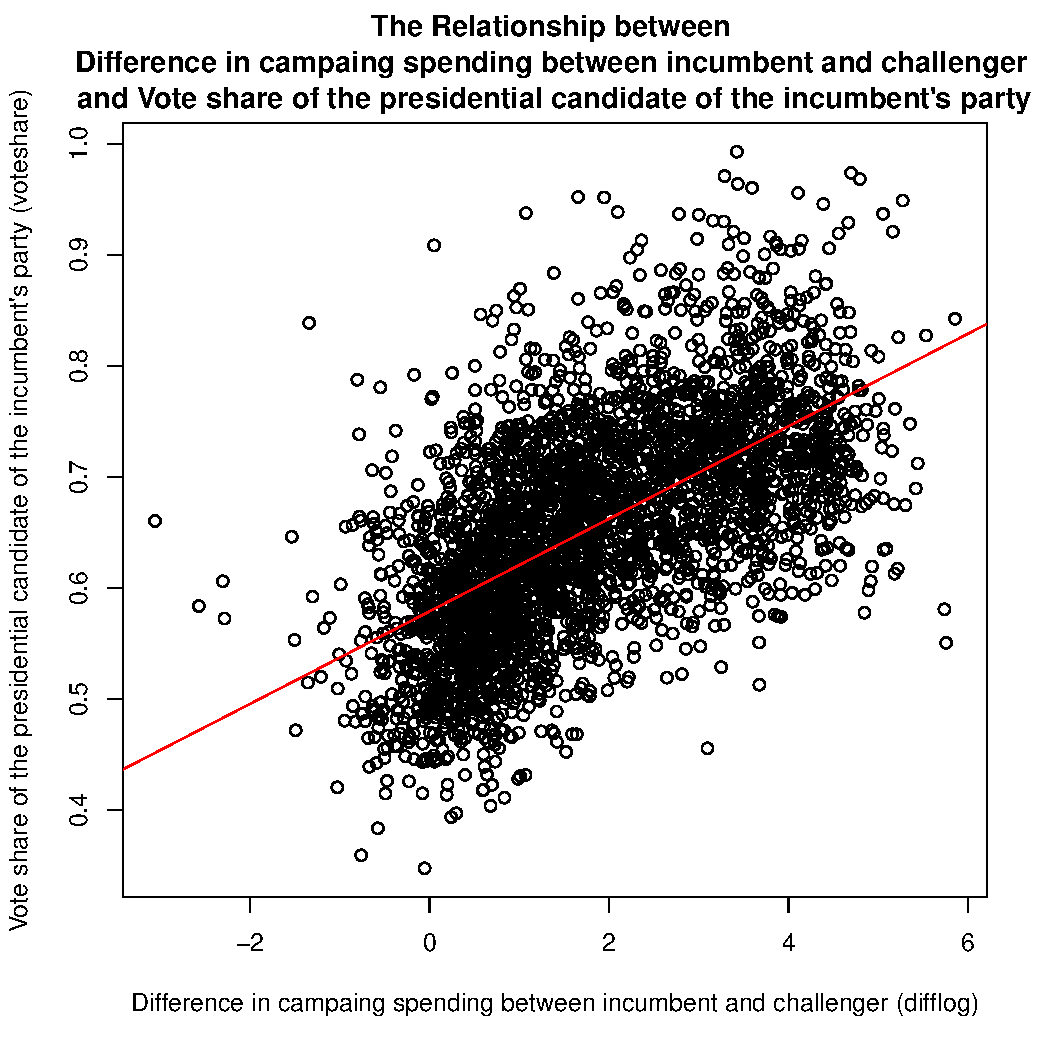
\includegraphics[width=.75\textwidth]{scatterplot_q1.pdf}
		\end{figure}
		
		\vspace{0.5cm}
		\noindent \textbf{Conclusion:} There is a positive relationship between \texttt{difflog} (the difference in campaign spending between incumbent and challenger) and \texttt{voteshare} (the incumbent's vote share).
		\vspace{0.5cm}
		
		\item Save the residuals of the model in a separate object.	\vspace{0.5cm}
		
		\noindent \textbf After execution of the regression model I can save the residuals of the model in a separate object by using residuals(). \vspace{0.5cm}
		
		\noindent \textbf{Code in R:}
		\lstinputlisting[language=R, firstline=58, lastline=59]{PS3_my answers_YK_23359606.R}  
		\vspace{.25cm}
		
		\noindent \textbf{Output: }
		\begin{verbatim}
1             2             3             
-0.0004227622 -0.0316840149 -0.0045514943  
4             5             6
0.0386688767  0.0355287965  0.0322832521 			
		\end{verbatim}  
		\vspace{.25cm}
		
		
		\item Write the prediction equation. \vspace{0.5cm}
		
		\noindent \textbf The formula of prediction equation is: \vspace{0.5cm}
		
$$ \text{Y}_i = \beta_0 + \beta_1 \text{X}_1_i + \beta_2 \text{X}_2_i + ... + \beta_k \text{X}_k_i +\epsilon_i $$
		
			\noindent \textbf Or \vspace{0.5cm}
			
			$$Y = Xb + e $$
		
		\noindent \textbf Getting the coefficients for writing the prediction equation. 
		\vspace{0.5cm}
		
		\noindent \textbf{Code in R:}
		\lstinputlisting[language=R, firstline=62, lastline=63]{PS3_my answers_YK_23359606.R}  
		\vspace{.25cm}
		
		\noindent \textbf{Output: }
		\begin{verbatim}
             Estimate   Std. Error   t value      Pr(>|t|)
	(Intercept) 0.57903071 0.0022513886 257.18826  0.000000e+00
	difflog     0.04166632 0.0009679924  43.04406 1.359767e-319
			
		\end{verbatim}  
		\vspace{.25cm}
		
		\noindent \textbf Writing the prediction equation. 
		\vspace{0.5cm}	
		
		\noindent \textbf{Code in R:}
		\lstinputlisting[language=R, firstline=65, lastline=65]{PS3_my answers_YK_23359606.R}  
		\vspace{.25cm}
		
		\noindent \textbf{Output: }
		\begin{verbatim}
		Prediction Equation: 
		voteshare = 0.5790307 + 0.04166632 * difflog
		\end{verbatim}  
		\vspace{1 cm}
		\vspace{1 cm}
		
		
		
	\end{enumerate}
	
\newpage

\section*{Question 2}
\noindent We are interested in knowing how the difference between incumbent and challenger's spending and the vote share of the presidential candidate of the incumbent's party are related.	\vspace{.25cm}
	\begin{enumerate}
		\item Run a regression where the outcome variable is \texttt{presvote} and the explanatory variable is \texttt{difflog}.	\vspace{0.5cm}
		
			\noindent \textbf Executing the regression model in which the incumbent's electoral success (\texttt{presvote}) is explained by the difference between incumbent and challenger's spending (\texttt{difflog}). Then I investigate the estimated coefficients of the model using summary(). \vspace{0.5cm}
		
		\noindent \textbf{Code in R:}
		\lstinputlisting[language=R, firstline=69, lastline=72]{PS3_my answers_YK_23359606.R}  
		\vspace{.25cm}
		
		\noindent \textbf{Output: }
				\begin{footnotesize}
		\begin{verbatim}
Residuals:     Min       1Q   Median       3Q      Max 
            -0.32196 -0.07407 -0.00102  0.07151  0.42743 
Coefficients:            
            Estimate Std. Error t value Pr(>|t|)    
(Intercept) 0.507583   0.003161  160.60   <2e-16 ***
difflog     0.023837   0.001359   17.54   <2e-16 ***
---
Signif. codes:  0 ‘***’ 0.001 ‘**’ 0.01 ‘*’ 0.05 ‘.’ 0.1 ‘ ’ 1
Residual standard error: 0.1104 on 3191 degrees of freedom
Multiple R-squared:  0.08795,	Adjusted R-squared:  0.08767 
F-statistic: 307.7 on 1 and 3191 DF,  p-value: < 2.2e-16
			
		\end{verbatim}  
				\end{footnotesize}
		\vspace{.25cm}
		
		\noindent \textbf{Conclusion:} Increasing the difference in campaing spending between incumbent and challenger by 1 unit, on average, will increase the incumbent's electoral success by 0.0238 units. The estimated coefficient is statistically diferentiable from zero at the  $\alpha=0.05$ level because the p-value $<$ 0.05 ($\approx $2e-16).
		\vspace{1 cm}
		
		\item Make a scatterplot of the two variables and add the regression line. 	\vspace{0.5cm}
		
		\noindent \textbf Making a scatterplot of the two variables and adding the regression line by using plot() and abline(). \vspace{0.5cm}
		
		\noindent \textbf{Code in R:}
		\lstinputlisting[language=R, firstline=75, lastline=84]{PS3_my answers_YK_23359606.R}  
		\vspace{0.25cm}
		

	\noindent Scatterplot 2 with the regression line.


\begin{figure}[h!]\centering
	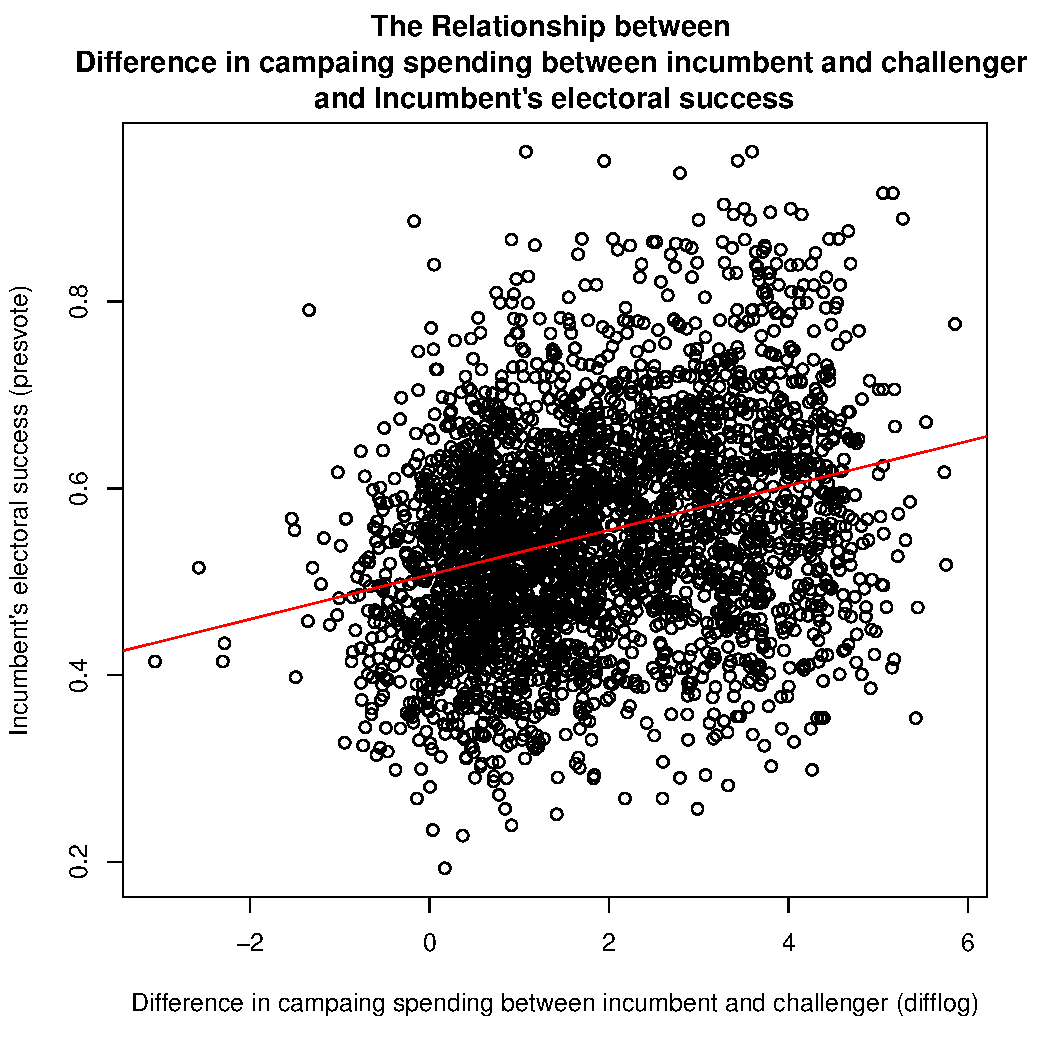
\includegraphics[width=.75\textwidth]{scatterplot_q2.pdf}
	\end{figure}

\vspace{0.5cm}

\noindent \textbf{Conclusion:} 
There is a positive relationship between \texttt{difflog} (the difference in campaign spending between incumbent and challenger) and \texttt{presvote} (the incumbent's electoral success).
\vspace{0.5cm}
		
		
		\item Save the residuals of the model in a separate object.	\vspace{0.5cm}
		
			\noindent \textbf After execution of the regression model I can save the residuals of the model in a separate object by using residuals(). \vspace{0.5cm}
		
		\noindent \textbf{Code in R:}
		\lstinputlisting[language=R, firstline=87, lastline=88]{PS3_my answers_YK_23359606.R}  
		\vspace{.25cm}
		
		\noindent \textbf{Output: }
		\begin{verbatim}
1            2            3            
0.005605594  0.037578519 -0.053134788 
4            5            6 
-0.052993694 -0.045842994  0.074339701
			
		\end{verbatim}  
		\vspace{.25cm}
		
		
		\item Write the prediction equation.
		
			\noindent \textbf Getting the coefficients for writing the prediction equation. 
		\vspace{0.5cm}
		
		\noindent \textbf{Code in R:}
		\lstinputlisting[language=R, firstline=91, lastline=92]{PS3_my answers_YK_23359606.R}  
		\vspace{.25cm}
		
		\noindent \textbf{Output: }
		\begin{verbatim}
            Estimate  Std. Error   t value     Pr(>|t|)
(Intercept) 0.50758333 0.003160529 160.60077 0.000000e+00
difflog     0.02383723 0.001358880  17.54182 7.681359e-66
			
		\end{verbatim}  
		\vspace{.25cm}
		
		\noindent \textbf Writing the prediction equation. 
				
		\noindent \textbf{Code in R:}
\lstinputlisting[language=R, firstline=94, lastline=94]{PS3_my answers_YK_23359606.R}  
\vspace{.25cm}

\noindent \textbf{Output: }
\begin{verbatim}
	Prediction Equation: 
	presvote = 0.5075833 + 0.02383723 * difflog
\end{verbatim}  
		\vspace{1 cm}
		
	\end{enumerate}
	
	\newpage	
\section*{Question 3}

\noindent We are interested in knowing how the vote share of the presidential candidate of the incumbent's party is associated with the incumbent's electoral success.
	\vspace{.25cm}
	\begin{enumerate}
		\item Run a regression where the outcome variable is \texttt{voteshare} and the explanatory variable is \texttt{presvote}.
			\vspace{0.5cm}
			
				\noindent \textbf Executing the regression model in which the vote share of the presidential candidate of the incumbent's party (\texttt{voteshare}) is explained by the incumbent's electoral success (\texttt{presvote}). Then I investigate the estimated coefficients of the model using summary(). \vspace{0.5cm}
			
			\noindent \textbf{Code in R:}
			\lstinputlisting[language=R, firstline=99, lastline=101]{PS3_my answers_YK_23359606.R}  
			\vspace{.25cm}
			
			\noindent \textbf{Output: }
							\begin{footnotesize}
			\begin{verbatim}
Residuals:     Min       1Q   Median       3Q      Max 
           -0.27330 -0.05888  0.00394  0.06148  0.41365 
Coefficients:            
           Estimate Std. Error t value Pr(>|t|)    
(Intercept) 0.441330   0.007599   58.08   <2e-16 ***
presvote    0.388018   0.013493   28.76   <2e-16 ***
---
Signif. codes:  0 ‘***’ 0.001 ‘**’ 0.01 ‘*’ 0.05 ‘.’ 0.1 ‘ ’ 1
Residual standard error: 0.08815 on 3191 degrees of freedom
Multiple R-squared:  0.2058,	Adjusted R-squared:  0.2056 
F-statistic:   827 on 1 and 3191 DF,  p-value: < 2.2e-16			
				
			\end{verbatim}  
							\end{footnotesize}
			\vspace{.25cm}
			
			\noindent \textbf{Conclusion:} Increasing the incumbent's electoral success by 1 unit, on average, will increase the vote share of the presidential candidate of the incumbent's party by 0.388 units. The estimated coefficient is statistically diferentiable from zero at the  $\alpha=0.05$ level because the p-value $<$ 0.05 ($\approx $2e-16).
			\vspace{1 cm}
			
		\item Make a scatterplot of the two variables and add the regression line. 
			\vspace{0.5cm}
			
		\noindent \textbf Making a scatterplot of the two variables and adding the regression line by using plot() and abline(). \vspace{0.5cm}
			
				\noindent \textbf{Code in R:}
			\lstinputlisting[language=R, firstline=104, lastline=113]{PS3_my answers_YK_23359606.R}  
			\vspace{.25cm}
			
\begin{center}
				\noindent Scatterplot 3 with the regression line.
\end{center}
			
			\begin{figure}[h!]\centering


				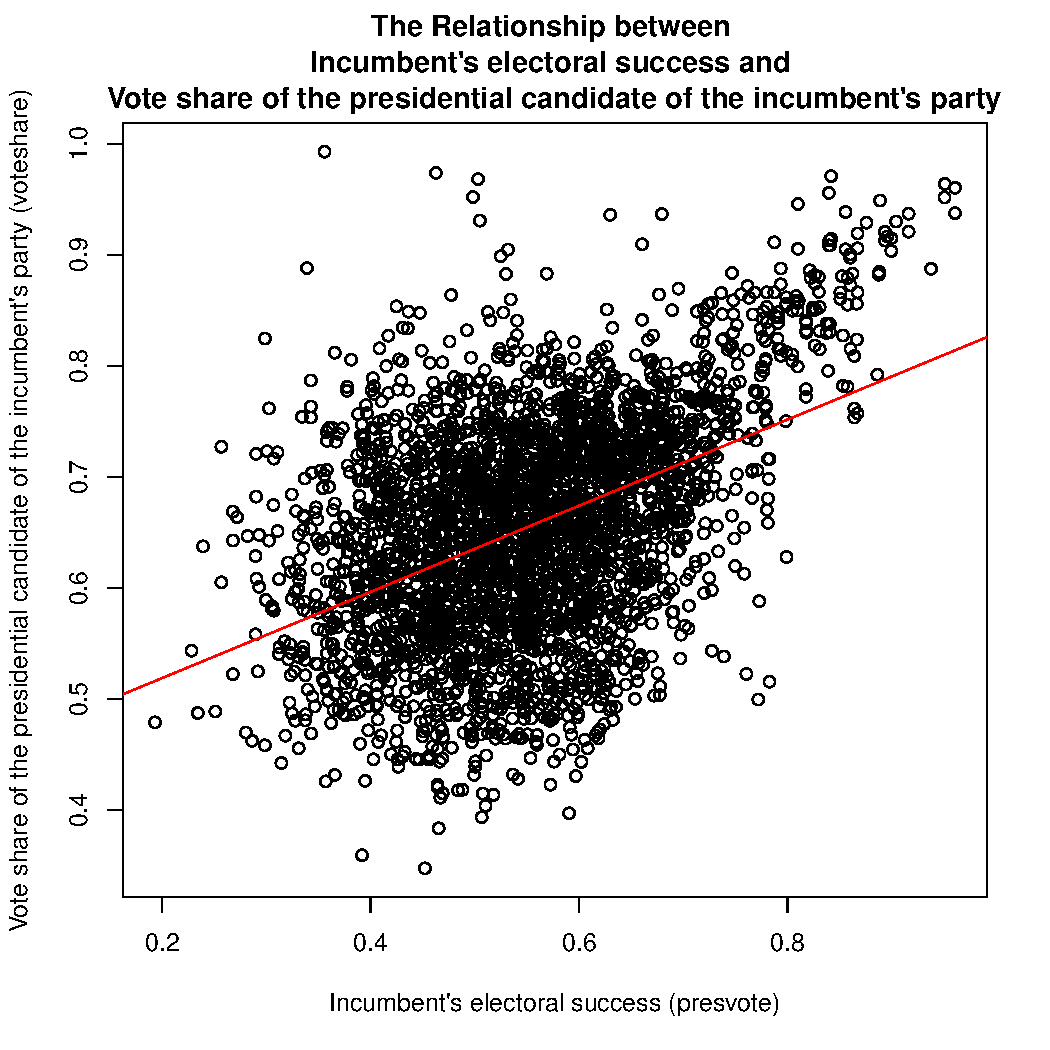
\includegraphics[width=.75\textwidth]{scatterplot_q3.pdf}
			\end{figure}
			
			\vspace{0.5cm}
			\noindent \textbf{Conclusion:} There is a positive relationship between \texttt{presvote} (the incumbent's electoral success) and \texttt{voteshare} (the vote share of the presidential candidate of the incumbent's party).
			\vspace{0.5cm}
			
		\item Write the prediction equation.
		
		\noindent \textbf Getting the coefficients for writing the prediction equation. 
		\vspace{0.5cm}
		
		\noindent \textbf{Code in R:}
		\lstinputlisting[language=R, firstline=116, lastline=117]{PS3_my answers_YK_23359606.R}  
		\vspace{.25cm}
		
		\noindent \textbf{Output: }
		\begin{verbatim}
             Estimate  Std. Error  t value      Pr(>|t|)
(Intercept) 0.4413299 0.007598612 58.08033  0.000000e+00
presvote    0.3880184 0.013493130 28.75674 6.586314e-162
			
		\end{verbatim}  
		\vspace{.25cm}
		
	\noindent \textbf Writing the prediction equation. 

\noindent \textbf{Code in R:}
\lstinputlisting[language=R, firstline=119, lastline=119]{PS3_my answers_YK_23359606.R}  
\vspace{.25cm}

\noindent \textbf{Output: }
\begin{verbatim}
Prediction Equation: 
voteshare = 0.4413299 + 0.3880184 * presvote
\end{verbatim}  

		\vspace{1 cm}
	\end{enumerate}
	

\newpage	
\section*{Question 4}
\noindent The residuals from part (a) tell us how much of the variation in \texttt{voteshare} is $not$ explained by the difference in spending between incumbent and challenger. The residuals in part (b) tell us how much of the variation in \texttt{presvote} is $not$ explained by the difference in spending between incumbent and challenger in the district.
	\begin{enumerate}
		\item Run a regression where the outcome variable is the residuals from Question 1 and the explanatory variable is the residuals from Question 2.	\vspace{0.5cm}
		
			\noindent \textbf Executing the regression model in which the residuals from Question 1 (\texttt{residuals1}) are explained by the residuals from Question 2 (\texttt{residuals2}). Then I investigate the estimated coefficients of the model using summary(). \vspace{0.5cm}
		
		\noindent \textbf{Code in R:}
		\lstinputlisting[language=R, firstline=125, lastline=127]{PS3_my answers_YK_23359606.R}  
		\vspace{.25cm}
		
		\noindent \textbf{Output: }
				\begin{footnotesize}
		\begin{verbatim}
Residuals:     Min       1Q   Median       3Q      Max 
             -0.25928 -0.04737 -0.00121  0.04618  0.33126 
Coefficients:                  
                   Estimate Std. Error t value Pr(>|t|)    
(Intercept)     -1.942e-18  1.299e-03    0.00        1    
st_residuals_q2  2.569e-01  1.176e-02   21.84   <2e-16 ***
---
Signif. codes:  0 ‘***’ 0.001 ‘**’ 0.01 ‘*’ 0.05 ‘.’ 0.1 ‘ ’ 1
Residual standard error: 0.07338 on 3191 degrees of freedom
Multiple R-squared:   0.13,	Adjusted R-squared:  0.1298 
F-statistic:   477 on 1 and 3191 DF,  p-value: < 2.2e-16	
			
		\end{verbatim}  
			\end{footnotesize}
		\vspace{.25cm}
		
		\noindent \textbf{Conclusion:} Increasing the residuals from Question 2 by 1 unit, on average, will increase the residuals from Question 1 by 0.257 units. The estimated coefficient is statistically diferentiable from zero at the  $\alpha=0.05$ level because the p-value $<$ 0.05 ($\approx $2e-16).
		\vspace{1 cm}
		
		\item Make a scatterplot of the two residuals and add the regression line. 	\vspace{0.5cm}
		
		\noindent \textbf Making a scatterplot of the two residuals and adding the regression line by using plot() and abline(). \vspace{0.5cm}
		
		\noindent \textbf{Code in R:}
		\lstinputlisting[language=R, firstline=130, lastline=139]{PS3_my answers_YK_23359606.R}  
		\vspace{.25cm}
		
\begin{center}
			\noindent Scatterplot 4 with the regression line.
\end{center}
		
		
		\begin{figure}[h!]\centering


			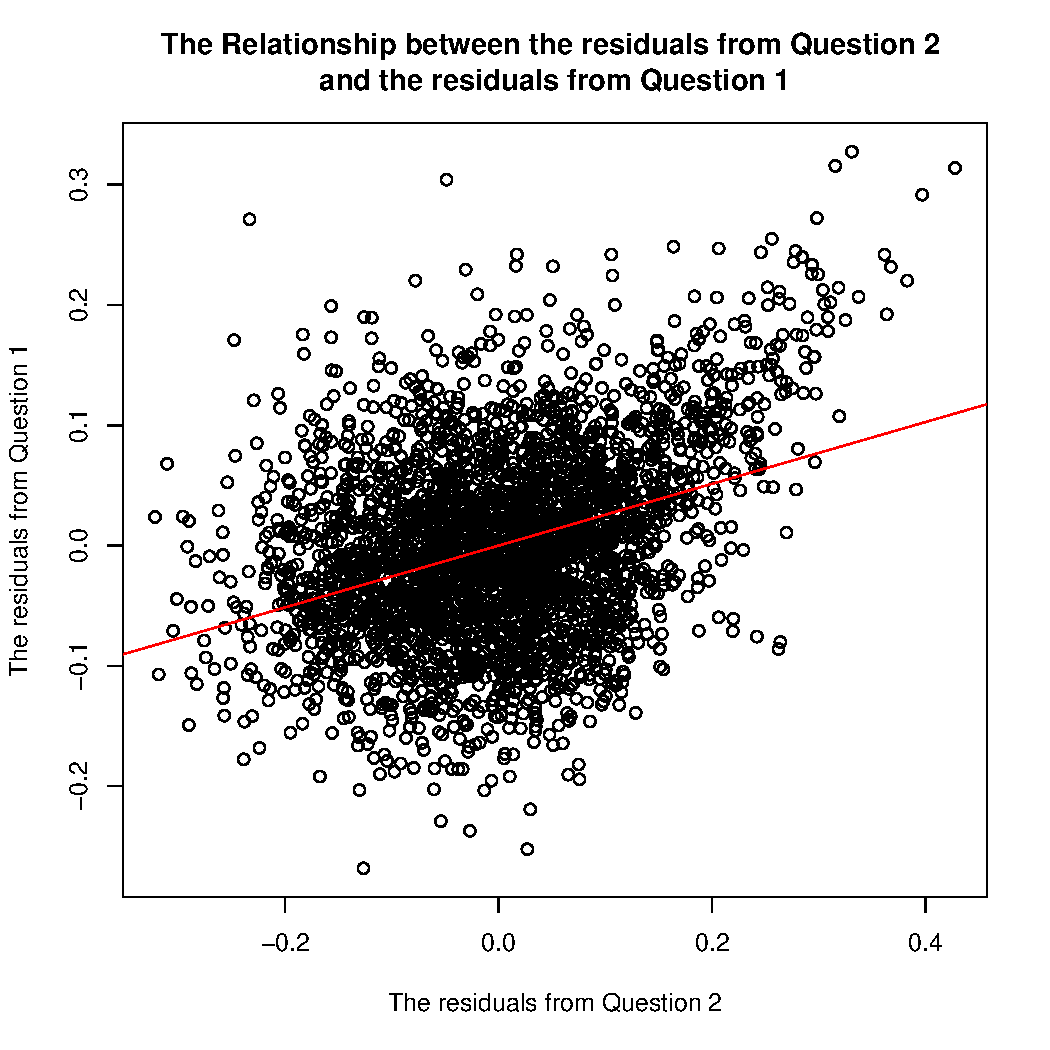
\includegraphics[width=.75\textwidth]{scatterplot_q4.pdf}
		\end{figure}
		
		\vspace{0.5cm}
		
		\noindent \textbf{Conclusion:} There is a positive relationship between residuals from Question 2 and residuals from Question 1.
		\vspace{0.5cm}
		
		\item Write the prediction equation.
		
		\noindent \textbf Getting the coefficients for writing the prediction equation. 
		\vspace{0.5cm}
		
		\noindent \textbf{Code in R:}
		\lstinputlisting[language=R, firstline=142, lastline=143]{PS3_my answers_YK_23359606.R}  
		\vspace{.25cm}
		
		\noindent \textbf{Output: }
		\begin{verbatim}
    (Intercept) st_residuals_q2   
-1.941539e-18    2.568770e-01 		
			
		\end{verbatim}  
		\vspace{.25cm}
		
		\noindent \textbf Writing the prediction equation. 
		\vspace{0.5cm}

		\noindent \textbf{Code in R:}
		\lstinputlisting[language=R, firstline=145, lastline=145]{PS3_my answers_YK_23359606.R}  
		\vspace{.25cm}

		\noindent \textbf{Output: }
		\begin{verbatim}
Prediction Equation: 
residuals_question1 = -1.941539e-18 + 0.256877 * residuals_question2
		\end{verbatim}  
		\vspace{1 cm}
		\end{enumerate}
	
	\newpage	

\section*{Question 5}
\noindent What if the incumbent's vote share is affected by both the president's popularity and the difference in spending between incumbent and challenger? 
	\begin{enumerate}
		\item Run a regression where the outcome variable is the incumbent's \texttt{voteshare} and the explanatory variables are \texttt{difflog} and \texttt{presvote}.	\vspace{0.5cm}
		
		\noindent \textbf Executing the regression model in which the vote share of the presidential candidate of the incumbent's party (\texttt{voteshare}) is explained by the difference in campaing spending between incumbent and challenger (\texttt{difflog}) and the incumbent's electoral success (\texttt{presvote}). Then I investigate the estimated coefficients of the model using summary(). \vspace{0.5cm}
		
		\noindent \textbf{Code in R:}
		\lstinputlisting[language=R, firstline=151, lastline=153]{PS3_my answers_YK_23359606.R}  
		\vspace{.25cm}
		
		\noindent \textbf{Output: }
				\begin{footnotesize}
		\begin{verbatim}
Residuals:     Min       1Q   Median       3Q      Max 
           -0.25928 -0.04737 -0.00121  0.04618  0.33126 
Coefficients:             
             Estimate Std. Error t value Pr(>|t|)    
(Intercept) 0.4486442  0.0063297   70.88   <2e-16 ***
difflog     0.0355431  0.0009455   37.59   <2e-16 ***
presvote    0.2568770  0.0117637   21.84   <2e-16 ***
---
Signif. codes:  0 ‘***’ 0.001 ‘**’ 0.01 ‘*’ 0.05 ‘.’ 0.1 ‘ ’ 1
Residual standard error: 0.07339 on 3190 degrees of freedom
Multiple R-squared:  0.4496,	Adjusted R-squared:  0.4493 
F-statistic:  1303 on 2 and 3190 DF,  p-value: < 2.2e-16
			
		\end{verbatim}  
			\end{footnotesize}
		\vspace{.25cm}
		
		\noindent \textbf{Conclusion:} Controlling the difference in campaing spending between incumbent and challenger, a 1 unit increase in the incumbent's electoral success is associated, on average, with 0.2568 increase in the vote share of the presidential candidate of the incumbent's party. 
		Controlling the incumbent's electoral success, a 1 unit increase in the difference in campaing spending between incumbent and challenger is associated, on average, with 0.0355 increase in the vote share of the presidential candidate of the incumbent's party.  The both estimated coefficients is statistically diferentiable from zero at the  $\alpha=0.05$ level because the p-value $<$ 0.05 ($\approx $2e-16).
		\vspace{1 cm}
		
		\item Write the prediction equation.	\vspace{0.5cm}
		
		\noindent \textbf Getting the coefficients for writing the prediction equation. \vspace{0.5cm}
		
		\noindent \textbf{Code in R:}
		\lstinputlisting[language=R, firstline=156, lastline=157]{PS3_my answers_YK_23359606.R}  
		\vspace{.25cm}
		
		\noindent \textbf{Output: }
		\begin{verbatim}
(Intercept)     difflog    presvote  
0.44864422  0.03554309  0.25687701 
			
		\end{verbatim}  
		\vspace{.25cm}
	
		\noindent \textbf Writing the prediction equation. 
		\vspace{0.5cm}	
		
		\noindent \textbf{Code in R:}
		\lstinputlisting[language=R, firstline=159, lastline=159]{PS3_my answers_YK_23359606.R}  
		\vspace{.25cm}
		
		\noindent \textbf{Output: }
		\begin{verbatim}
Prediction Equation: 
voteshare = 0.4486442 + 0.03554309 * difflog + 0.256877 * presvote
		\end{verbatim}  
		\vspace{1 cm}
		
		\item What is it in this output that is identical to the output in Question 4? Why do you think this is the case?  \vspace{0.5cm}
		
		\noindent The prediction equation from Question 4 is: 
					\begin{verbatim}
		residuals_question1 = -1.941539e-18 + 0.256877 * residuals_question2
	\end{verbatim}  
		
		The prediction equation from Question 5 is: 
			\begin{verbatim}
		voteshare = 0.4486442 + 0.03554309 * difflog + 0.256877 * presvote
	\end{verbatim}  
	
	\noindent The identical part in the two preditiction equations is the estimated coefficient 0.256877. I think this is case because when we do assumption about linear regression we assume that there is an error:
	$$ \text{Y}_i = \alpha + \beta \text{X}_i + \epsilon_i $$
	
	\noindent In Question 4 we have written a prediction equation where: 
	$$ \text{residuals}_1= -1.941539e-18  + 0.256877*\text{residuals}_2 \approx $$
	$$  \approx 0 + 0.256877*\text{residuals}_2 = 0.256877*\text{residuals}_2 $$ 
	
	\noindent Having the linear relationship between variables \texttt{voteshare} and \texttt{difflog} such as:
	$$ \text{voteshare} = \alpha + \beta * \text{difflog} + \text{residuals}_1   $$
	\noindent which we can rewrite as an equation:
	
	$$ \text{voteshare}  = \alpha + \beta * \text{difflog} + 0.256877*\text{residuals}_2   $$
	
	\noindent Thus, making assupmtion about having error, we include in the regression model the another predictor, in this case  \texttt{residuals2}, and this predictor is highly correlated with variable \texttt{presvote}. We see the same coefficient in the prediction equation from Question 5:
	$$ \text{voteshare}  = 0.4486442 + 0.03554309 * \text{difflog} + 0.256877*\text{presvote}   $$
	 
	\vspace{0.5 cm}
	
	\noindent Checking the correlation coefficient between \texttt{presvote} and \texttt{residuals2} in R:
	
	\noindent \textbf{Code in R:}
	\lstinputlisting[language=R, firstline=165, lastline=165]{PS3_my answers_YK_23359606.R}  
	\vspace{.25cm}
	 
	 
	 	\noindent \textbf{Output: }
	 \begin{verbatim}
[1] 0.9550126
	 \end{verbatim}  
	 \vspace{1 cm}
	 

	\end{enumerate}




\end{document}
